\chapter{The ALICE experiment at the LHC}
\label{chap:chap3}

\section{The Large Hadron Collider}
\label{sec:LHC}
The Large Hadron Collider (LHC), with a circumference of 27 km, 
is the world largest and most powerful particle collider, built by the 
European Organisation for Nuclear Research (CERN) from 1998 to 2008. 
It is placed in the tunnel of the previous Large Electron Positron collider, at a depth between 50 and 175 m underground.
The LHC accelerator chain is shown in Fig.~\ref{fig:imageLHC}. The first stage 
of the acceleration takes place on the Linac2, a linear accelerator with an 
output proton energy of 50 MeV. The proton-booster synchrotron (PSB) increases 
the energy to 1.4 GeV, injecting into the proton synchrotron (PS). This accelerates the
 beam to 26 GeV and injects it into the super proton synchrotron (SPS), out of which 
 450 GeV protons are eventually injected into the LHC for the start of the ramp up to 
 the energy of 7 TeV. At the nominal configuration, LHC accelerates protons grouped in 2808 bunches per beam, each bunch 
 containing up to $1.15^{11}$ protons. The beam is bent along the circular LHC 
 path by 1232 superconducting dipoles and controlled and focused by other 
 600 smaller magnets. The design and construction of the dipoles was the most 
 technologically challenging part of the accelerator. To achieve the required bending power, 
 the dipole field should be on average B $\sim$ 8.3 Tesla. The coils are made of 
 NiTi superconducting cable, kept at T = 1.9 K by superfluid liquid He. They are 
 15 m long, weigh 35 tonnes and store in their magnetic field 7 MJ of energy, for a total of 10 GJ in the full ring.\\
The nominal instantaneous luminosity for pp collisions, with a bunch crossing every 25 ns, is of $10^{34} {\rm s}^{-1} {\rm cm}^{-2}$; for 
Pb-Pb collisions it is about $10^{27} {\rm s}^{-1} {\rm cm}^{-2}$. Since September 2008, 
the four main experiments (ALICE, ATLAS, CMS and LHCb) collected data with pp
 collisions at $\s=900, 2.36, 2.76, 5, 7, 8$ and 13 TeV, 
 Pb-Pb collisions at $\sNN=2.76$ and 5.02 TeV, Xe-Xe collisions at $\sNN=5.44$ TeV and p-Pb collisions at $\sNN=5.02$ TeV.

\begin{figure}[!t]
\centering
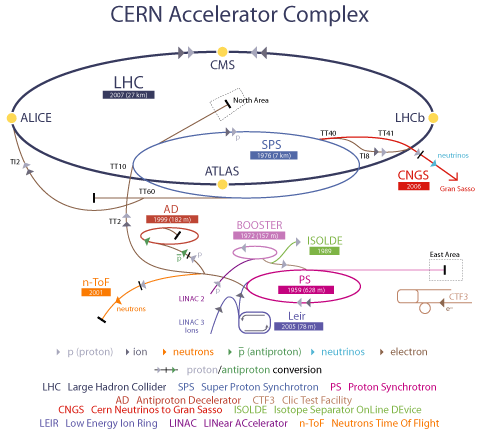
\includegraphics[width=12cm]{FigCap3/CERN_Accl_Complex.png}
\caption{Layout of the full CERN accelerator complex, including all elements of the LHC injector chain.}
\label{fig:imageLHC}
\end{figure} 
\section{The ALICE experiment}
\label{sec:ALICE}
ALICE (A Large Ion Collider Experiment)~\cite{Abelev:2014ffa} is an experiment 
at the LHC optimised for the study of QCD matter
created in high-energy collisions between heavy nuclei.
The aim of ALICE is the study of the behaviour of matter at high densities and temperatures 
and at nearly zero baryo-chemical potential. 
The major challenge that the detector project had faced was the large number of 
particles created in Pb-Pb collisions. Moreover, the study of the QGP requires to reconstruct tracks down to
low momenta and identify them on a wide momentum range.
For this reason, ALICE detectors were designed to have a 
high granularity, a low transverse momentum threshold $\pt^{\rm min} \sim 0.15 $ 
$\Gevc$ and good particle identification capabilities up to 20 $\Gevc$.
The apparatus consists of three main parts: 
\begin{itemize}
\item \textbf{central barrel}, contained within the large magnet producing a moderate solenoidal 
field of B = 0.5 T in nominal running conditions and composed of detectors devoted to the reconstruction of charged particles, photons
and jets and covering the pseudo-rapidity range -0.9 $< \eta <$ 0.9 over the 
full azimuth. They are the Inner Tracking System (ITS), optimised for vertex 
reconstruction and tracking; a cylindrical Time Projection Chamber (TPC),
 surrounding the ITS, that is the main detector for tracking and provides also particle identification; a 
 Transition Radiation Detector (TRD), designed for electron identification; 
 a Time Of Flight (TOF) detector, that provides pion, proton and kaon 
 identification; a Photon Spectrometer (PHOS); an Electromagnetic 
 Calorimeter (EMCal) and a Di-Jet Calorimeter (DCal), a High-Momentum Particle IDentification (HMPID) 
 and the ALICE Cosmic Ray Detector (ACORDE);
\item \textbf{forward muon spectrometer}, dedicated to the study of 
muons in the pseudo-rapidity range $2.5< \eta < 4.0$;
\item \textbf{the forward detectors}, which include the Photon Multiplicity Detector 
(PMD) and the silicon Forward Multiplicity Detector (FMD), dedicated to the 
measurement of photons and charged particles around $|\eta| \sim 3$, respectively; 
the quartz Cherenkov T0 detector, which delivers the time and the longitudinal
 position of the interaction; the plastic scintillator V0 detector, which measures 
 charged particles at -3.7 $< \eta <$ -1.7 and 2.8 $< \eta <$ 5.1, and is mainly used
  for triggering and for the determination of centrality and event plane angle in 
  Pb-Pb collisions; the Zero Degree Calorimeter (ZDC) also used for determination of centrality.
\end{itemize}
The layout of ALICE set-up is shown in Fig.~\ref{fig:imageALICE}. 
\begin{figure}[!t]
\centering
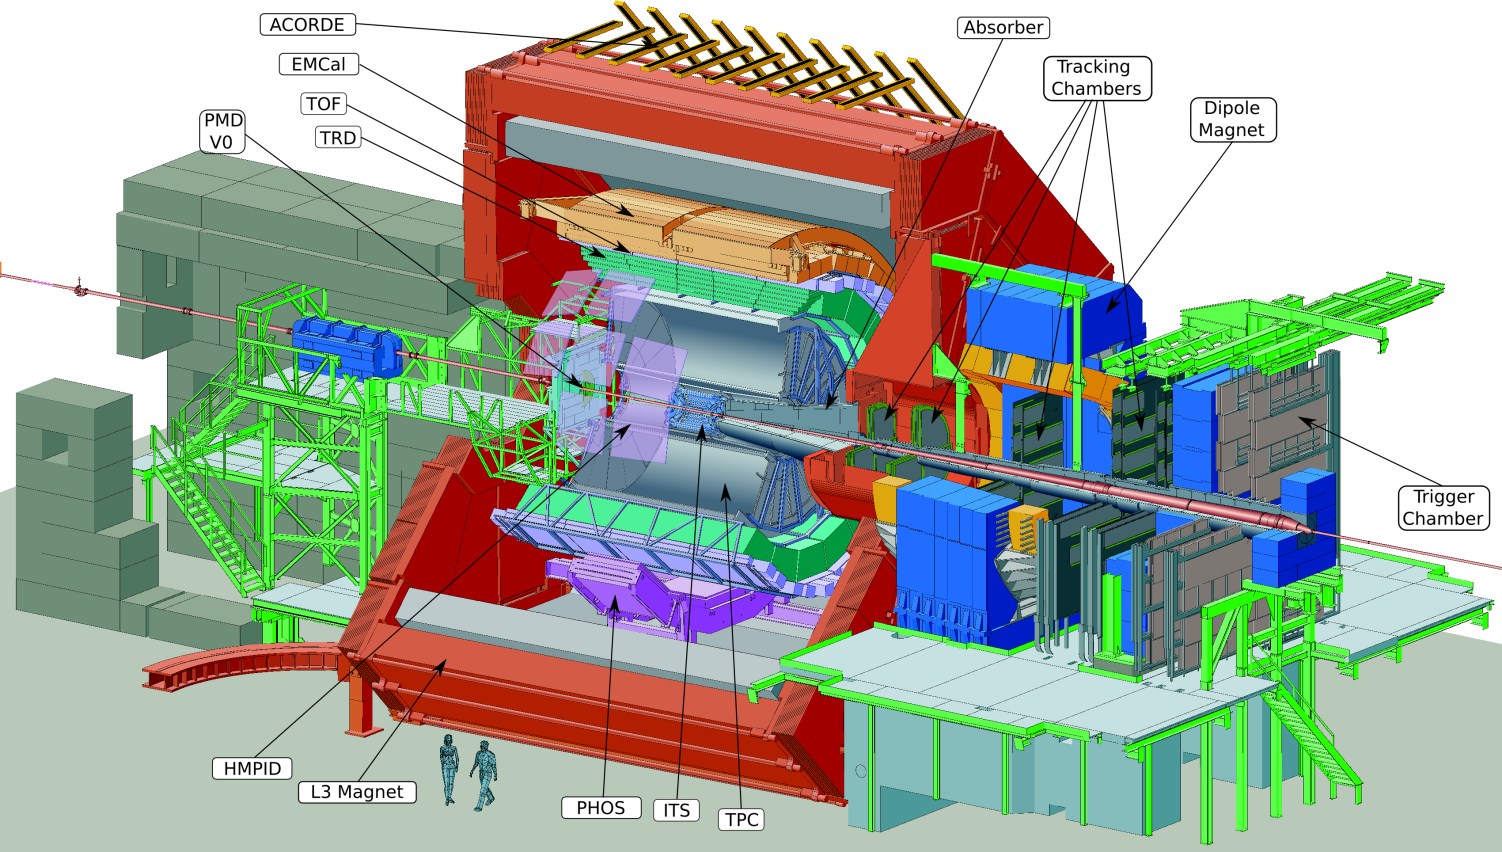
\includegraphics[width=12cm]{FigCap3/alice.png}
\caption{Picture of the ALICE experiment detectors.}
\label{fig:imageALICE}
\end{figure}
ALICE apparatus has overall dimensions of 16 x 16 x 26 m$^3$ and a total 
weight of $\sim$10000 t. The maximum pp interaction rate at which all ALICE 
detectors can be safely operated is around 700 kHz. Typical luminosity values 
for the ALICE pp data taking range from \textit{L} $\sim 10^{29}{\rm s}^{-1}{\rm cm}^{-2}$ 
to \textit{L} $\sim 10^{31}{\rm s}^{-1}{\rm cm}^{-2}$.
In the following sections, the detectors of ALICE used in the analyses presented in this thesis and their 
performance will be described. For information on the other detectors more details can be found in~\cite{Aamodt:2008zz}.

\subsection{Magnet}
\label{sec:Magnet}
The magnet used in ALICE was constructed for the L3 experiment at LEP and 
it produces a moderate solenoidal magnetic field (B $<$ 0.5 T). In the choice 
of the magnetic field two aspects must be considered: the magnet has to be intense 
enough to bend the particle trajectory and allow a good track-momentum resolution, 
but has to permit the reconstruction of low 
momentum particles. The lower momentum that allows reconstruction of the track 
with the ALICE magnet is given by $p_{\rm cutoff}=$ 0.3$\,$B$\,$R $\sim 0.2\,\Gevc$, 
where B is the magnetic field in Tesla and R is the minimum radius for a particle to 
traverse the entire TPC, whose external radius is R$_{\rm ext}=$ 2.5 m.
Tracks with lower momentum can be reconstructed using the Inner tracking System, as discussed
in the next sections.

\begin{figure}[!t]
\centering
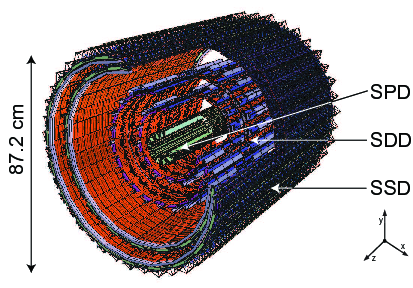
\includegraphics[width=8cm]{FigCap3/figures_its-rf-2.png}
\caption{View of the six silicon layers of the Inner Tracking System}
\label{fig:image2}
\end{figure}

\subsection{Inner Tracking System (ITS)}
\label{sec:ITS}
The Inner Tracking System is one of the central barrel detectors used for track 
reconstruction, primary and secondary vertex finding and Particle Identification (PID).
It is composed by six cylindrical layers of silicon detectors placed 
coaxially around the beam vacuum tube (Fig.~\ref{fig:image2}). The layers are located 
at radii between 39 mm and 430 mm and cover the pseudo-rapidity range 
$|\eta|<0.9$. The two innermost layers are made of Silicon Pixel Detectors (SPD). 
The pseudo-rapidity coverage of the SPD inner layer is $|\eta|<1.95$ for particles produced at $\zVtx=0$. 
The two middle layers are made of Silicon Drift Detectors (SDD) 
and two outer layers of Silicon micro-Strip Detectors (SSD).
Its basic functions are~\cite{ITS-TDR}:
\begin{itemize}
\item determination with high precision of primary vertex position (interaction point) and reconstruction of secondary vertices 
of charm, beauty and hyperon decays,
\item improvement of the momentum and angle measurements of the TPC,
\item recover particles that are not tracked in the TPC due to acceptance limitation (very low momentum particles
not reaching the TPC and high momentum particles crossing the inactive areas between adjacent TPC chambers).
\end{itemize}
All the ITS detectors were carefully optimised to minimise their radiation 
 length, achieving 1.1\% per layer, the lowest value among all the current LHC experiments~\cite{ITS-TDR}. 
The resolution of the track impact parameter is determined by the spatial resolution of 
the ITS detectors. The ITS detectors have a spatial resolution of a few tens of 
$\mu$m in the $r\varphi$ plane, with the best precision (12  $\mu$m) for the 
innermost detectors equipped with SPD. The left and the right panels of Fig.~\ref{fig:VtxResolDCAResol}, that will be discussed
 in Sec.~\ref{sec:tracking}, show respectively the resolution on the final vertex position in transverse coordinates and on the impact parameter
in the transverse plane. \\
 
 \begin{figure}[!h]
\centering
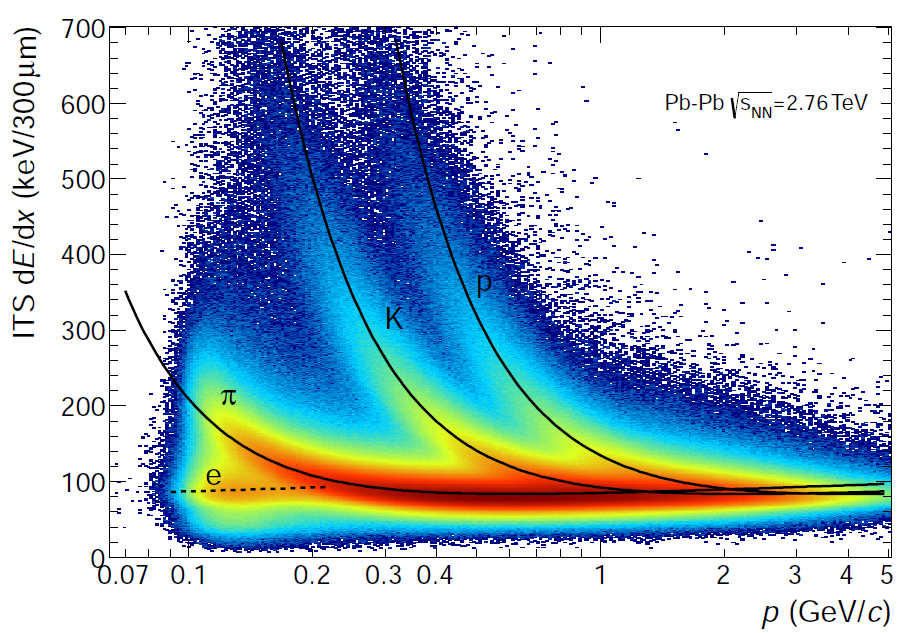
\includegraphics[width=.65\textwidth]{FigCap3/ITSpid.png}
\caption{Distribution of the energy-loss signal in the ITS as a function of momentum. The lines show the parameterisations of the expected mean energy loss.}
\label{fig:imagePIDITS}
\end{figure}

 The four outer layers provide analogue read-out and for this reason they 
 can be used for particle identification (PID) via d$E$/d$x$ measurements for 
 low-$\pt$ particles. The measured cluster charge in each of the four layers with PID capabilities is normalised to the path length
 in the silicon active volume, 
 which is calculated from the reconstructed track parameters, to obtain a d$E$/d$x$ 
 value for each layer. A single d$E$/d$x$ value is then calculated with a truncated mean of
 the values from the four layers, to assure that
 the d$E$/d$x$ peak shape is Gaussian. 
  The resolution $\sigma$ on the d$E$/$x$ is of about 10\% and it provides kaon-pion
 separation at 1$\sigma$ level for $\pt \lesssim 0.7 \, \Gevc$ and proton/pion separation 
 for $\pt \lesssim 1.2 \, \Gevc$.
 An example of the distribution of the measured truncated mean values of energy loss 
 per path unit as a function of track momentum in the ITS is shown 
 in Fig.~\ref{fig:imagePIDITS}. 
 \begin{figure}[!h]
\centering
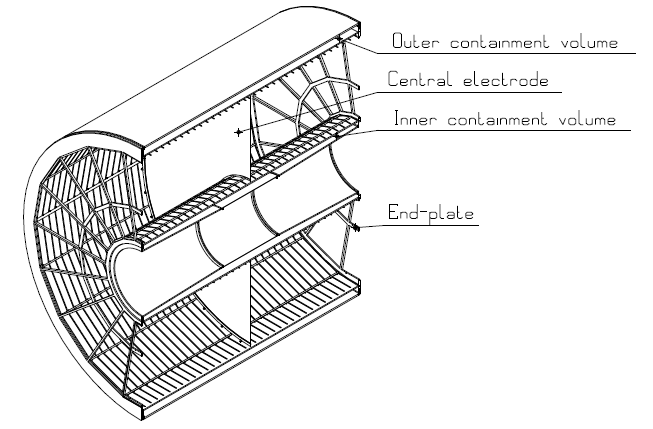
\includegraphics[width=.6\textwidth]{FigCap3/TPC.png}
\caption{A view of the ALICE Time-Projection Chamber detector.}
\label{fig:imageTPC}
\end{figure}

\subsection{Time Projection Chamber (TPC)}
\label{sec:TPC}
The TPC is the only device which can provide good tracking
performance up to track densities of 8000 charged particles per unit of rapidity, 
which were foreseen to be produced in Pb-Pb collisions at the LHC at the time when
ALICE was designed~\cite{Dellacasa:451098}. 
It has a cylindrical shape with inner and outer radius of 80 and 250 cm, 
respectively, and an overall length in the beam direction of 500 cm. The minimum  
inner radius of the TPC was determined by the maximum acceptable hit density. 
The outer radius was defined by the minimum length required for a d$E$/d$x$ resolution 
better than 10\%. At smaller radii (and larger track densities), tracking is taken over 
by the ITS. The TPC covers an acceptance of $|\eta|<0.9$. The TPC is a chamber full of 
high-purity gas to transport ionisation electrons over long distances (2.5 m) towards the read-out end-plates. 
It is composed by a central high-voltage (HV) electrode which divides the 
gas volume into two symmetric drift regions, and two opposite axial potential degraders to
create a highly uniform electrostatic field of up to 400 V/cm (Fig.~\ref{fig:imageTPC}).
Charged particles traversing the gas form a ionisation trace that will move at constant 
velocity towards one of the two end-plates. The density of ionisation depends on the velocity and mass of the particle.
Once on the end-plate, readout chambers allow to amplify and register the signals 
of particle tracks. The end-plates are segmented into 18 trapezoidal sectors 
and equipped with multi-wire proportional chambers covering an overall active area of 32.5 $m^2$.
The original mixture of gas was composed by 90\% Ne, 10\% ${\rm CO}_2$; successively a further 5\% of N$_2$
was added. During 2015-2016, the Ar replaced the Ne in the mixture.
 \begin{figure}[!h]
\centering
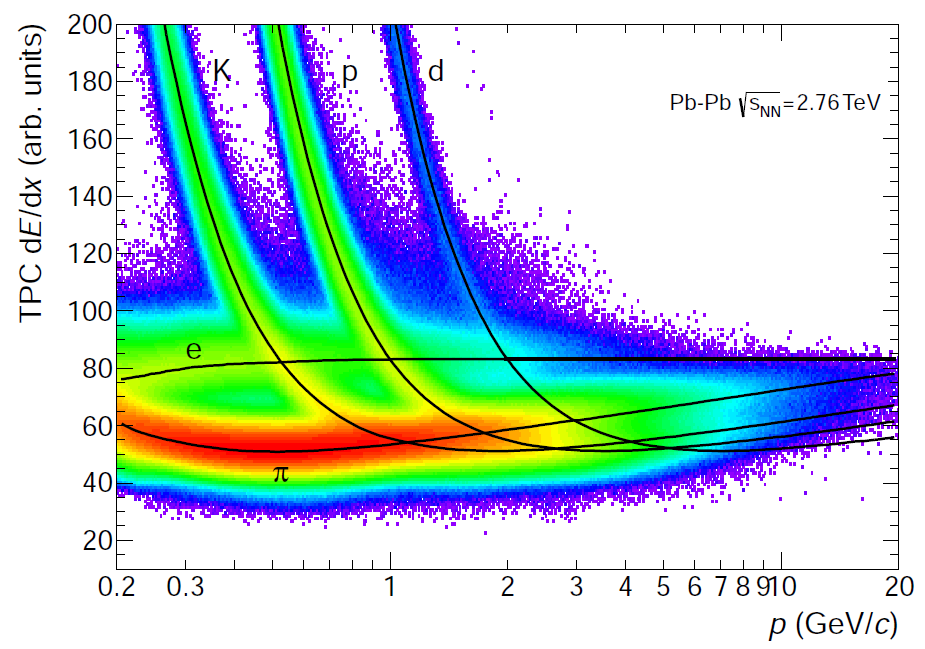
\includegraphics[width=.65\textwidth]{FigCap3/TPCpid.png}
\caption{Distribution of the energy-loss signal in the TPC as a function of momentum. The lines show the parameterisations of the expected mean energy loss.}
\label{fig:imagePIDTPC}
\end{figure}
The TPC is the main detector for track reconstruction (see Sec.~\ref{sec:tracking}). 
It is used for measurements of the charged-particle 
momenta, with a resolution better than 2.5\% for electrons with momentum 
of about 4 $\Gevc$, and for particle identification via d$E$/d$x$.\\


Particle Identification is performed over a wide momentum range. It is made by 
simultaneously measuring the specific energy loss, the charge and the momentum of the 
particles traversing the detector gas. The maximum number of clusters associated to a track in the TPC 
is 159 and the d$E$/d$x$ value of the track is determined using a truncated mean.
The d$E$/d$x$, described by the Bethe Bloch formula,
is parameterised by a function proposed by ALEPH Collaboration~\cite{Rolandi:2008qla}:
\begin{equation}
f(\beta_\gamma) = \frac{P_1}{\beta^{P_4}} \Big ( P_2 - \beta^{P_4} - {\rm ln}\Big (   P_3 + \frac{1}{(\beta_\gamma)^{P_5}} \Big )   \Big ),
\end{equation}
where $\beta$ is the particle velocity, $\gamma$ is the Lorentz factor, and $P_{1-5}$ are fit parameters. 
The measured d$E$/d$x$ as a function of the track momentum measured in TPC is
shown in Fig.~\ref{fig:imagePIDTPC}. The lines correspond to the parametrisation. 
A clear separation among the different particle species
is observed for $\pt \lesssim 1 \, \Gevc$, which allows for a PID on a track-by-track basis. At higher $\pt$ the separation of the species is still feasible 
on a statistical basis via multi-Gaussian fits. The PID resolution is about 5.2\% in 
pp collisions and 6.5\% in the 5\% most central Pb-Pb collisions. Thanks to the d$E$/d$x$ resolution, 
particle ratios can be measured in the relativistic rise region at $\pt$ up to $\approx 20\, \Gevc$.
 \begin{figure}[!h]
\centering
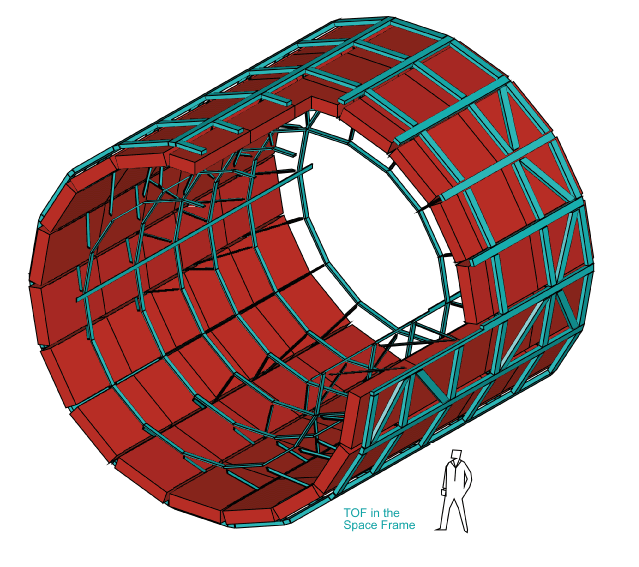
\includegraphics[width=.5\textwidth]{FigCap3/TOFCylinder.png}
\caption{A view of the ALICE Time-Of-Flight detector.}
\label{fig:imageTOF}
\end{figure}

\subsection{Time-Of-Flight (TOF)}
\label{sec:TOF}
The TOF detector is a large area array of Multigap Resistive Plate Chambers (MRPC), 
positioned at radial distance of 370-399 cm from the beam axis. It has a cylindrical 
shape, covering polar angles between 45 and 135 degrees over the full azimuth. 
The TOF has a modular structure with 18 sectors in $\varphi$ (Fig.~\ref{fig:imageTOF}); each 
of these sectors is divided into 5 modules along the beam direction. 
This detector is entirely devoted to particle identification. 
The ionisation produced by any particle crossing the MRPCs starts a gas avalanche 
which generates the observed signal. The TOF identifies the particle species via a measure of the time of flight 
inside the chambers. Let us consider the following relation:
\[
m = p \sqrt{\frac{t^2_{\rm TOF}}{L^2}-1}
\]
where $m$ is the mass of the particle, $p$ the momentum, $t_{\rm TOF}$ the time-of-flight and 
$L$  the track length. It can be shown that the $\sigma_m/m$ resolution, at relatively high
 momenta, it is influenced much more by the errors on the time-of-flight and track length 
 measurements than by error on the momentum determination.
 The time of collision, which constitutes the start time for the time-of-flight measurement,
 is obtained on an event-by-event basis either using the particle arrival times
 at the TOF, or the information from the T0 detector, or a combination of the two~\cite{Adam:2016ilk}. 
 The T0 detector is composed by two arrays of
Cherenkov counters, T0A and T0C, located at apposite sides of the interaction point at 
$-3.28 < \eta < - 2.97$ and $4.61 < \eta < 4.92$. It has a time resolution of 20-25 ps
 in Pb-Pb collisions and $\sim 40$ ps in pp collisions.
 The TOF resolution is 80 ps for pions with a momentum around 1 $\Gevc$, in 0-70\% Pb-Pb collisions.
This value includes the detector resolution, the contribution from electronics and the uncertainty
on the start time of the event.
It provides PID in the intermediate momentum range, allowing for pion/kaon separation at 3$\sigma$ level
up to $\pt \approx 2.5 \,\Gevc$  and kaon/pion separation up to $\pt \approx 4 \,\Gevc$.
Figure \ref{fig:TOFpid} shows the distribution of the measured velocity $\beta$ as a function of momentum (measured by TPC). 
The background is due to tracks that are incorrectly matched to TOF hits in high-multiplicity Pb-Pb collisions.
\begin{figure}[!h]
\centering
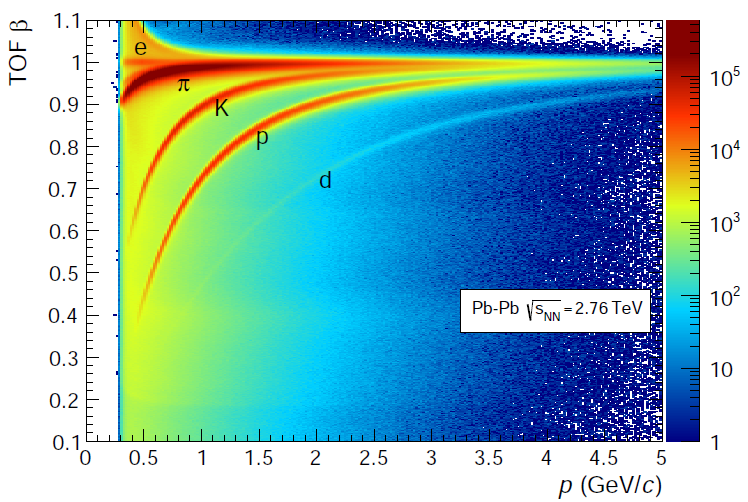
\includegraphics[width=.7\textwidth]{FigCap3/TOFpid.png}
\caption{Distribution of $\beta$ velocity measured by the TOF detector as a function of momentum for particles reaching the
TOF in Pb-Pb interactions.}
\label{fig:TOFpid}
\end{figure}


\subsection{V0 Detector} 
\label{sec:V0}
The V0 detector is made of two arrays of scintillator counters, V0A and V0C, positioned on both sides of 
the interaction point. The V0A detector is located at 340 cm distance from the nominal interaction point position, 
along the beam axis, on the side opposite to the muon spectrometer,
whereas V0C is fixed to the front face of the hadronic absorber, 90 cm from the nominal interaction point. They cover
the pseudo-rapidity ranges $2.8 < \eta < 5.1$ (V0A) and $-3.7 < \eta < -1.7$ (V0C) and are segmented
into 32 individual counters each distributed in four radial rings and 8 azimuthal sectors. 
The V0 provides a minimum bias trigger as well as high-multiplicity triggers for the central barrel detectors and
  can be used to estimate the centrality of the collision based on the energy deposited in the V0 scintillator tiles.
Furthermore, it is used for beam-gas background rejection (see Sec.~\ref{sec:BkgRejection}).


\subsection{Zero Degree Calorimeter (ZDC) Detector} 
\label{sec:ZDC}
The ZDC provides a measure of the energy carried in the forward direction (at 0$^\circ$ relative
to the beam direction) by non-interacting (spectator) nucleons. This quantity is
useful to estimate the centrality of the event. Typically the beams are deflected by means 
of two separation dipoles located at about 65 m distance from the interaction point (IP). These magnets will also deflect the spectator
 protons, separating them from the spectator neutrons, which fly away at 0$^\circ$. 
Two sets of ZDCs are placed at about 115 m distance from the 
 interaction point on both sides of the interaction point. Each set is constituted by one 
 calorimeter for neutron detection (ZN), positioned between the two 
 beam vacuum tubes to intercept the spectator neutrons, and one for proton detection (ZP), placed externally 
 to the outgoing beam, to collect the spectator protons. 
  The hadronic ZDCs are quartz-fibre sampling calorimeters. The shower generated by incident
particles in a dense absorber (tungsten for ZN and brass for ZP) produces 
Cherenkov radiation in quartz fibres (the active material) interspersed in the absorber.
The two sets of ZDCs are complemented by the information of two small 
electromagnetic calorimeters (ZEM), located at 7.5 m from the interaction
 point, to detect the  energy of particles emitted at forward rapidity (mainly photons generated from $\pi^0$ decays).




\section{The ALICE Trigger System and Data Aquisition}
\label{sec:trigger}
ALICE has a two-layer trigger architecture~\cite{Fabjan:684651}. The low-level trigger is a 
hardware trigger called Central Trigger Processor (CTP). The High-Level trigger (HLT)
 is implemented as a pure software trigger. 
The ALICE Central Trigger Processor (CTP) is designed to combine and synchronise 
information from all the triggering detectors in ALICE and informations about the LHC filling scheme and
bunch crossing, and to send the correct sequences
 of trigger signals to all detectors. Since the ALICE 
 experiment has to collect data in pp (p-Pb) and Pb-Pb collisions, the trigger system was optimised 
 for these two types of collisions. The HLT allows the implementation of sophisticated 
 logic for the triggering. While the CTP governs the readout of the sub-detectors, the 
 HLT receives a copy of the data read out from the sub-detectors and processes it.

\subsection{The Central Trigger Processor (CTP)}
\label{sec:CTP}
The hardware trigger combines informations from sub-detectors to decide whether or 
not to write an event on disk. The CTP evaluates trigger inputs from the trigger detectors every machine clock cycle ($\sim25$ ns). 

The trigger inputs are divided into three different levels:
\begin{itemize}
\item L0 level: the Level 0 trigger decision (L0) is made $\sim 0.9\, \mu$s after the 
collision using V0, T0, EMCal, PHOS, and MTR. The trigger requirement can be 
simply the input of one detector or a logical condition based on the trigger 
inputs of different trigger detectors.
\item L1 level: the events accepted at L0 are further evaluated by the Level 1 (L1) 
trigger algorithm in the CTP. The L1 trigger decision is made $\sim 6.5\, \mu$s after L0. 
The latency is caused by the computation time (TRD and EMCal) and propagation times 
(ZDC, 113 m from IP2). The L0 and L1 decisions, delivered to the detectors with a 
latency of about 300 ns, trigger the buffering of the event data in the detector front-end electronics. 
\item L2 level: the Level 2 (L2) decision, taken after about 100 $\mu$s corresponding to the 
drift time of the TPC, triggers the sending of the event data to DAQ and, in parallel, to the High Level Trigger system (HLT). 
L2 can be used to reject events with multiple collisions (pile-up) in different bunch crossings occurring
in the TPC readout time.
\end{itemize}
Information about the LHC bunch filling scheme is used by CTP to suppress the background. 
The information about the bunch crossing, regarding the arrival of bunches from both A-side and C-side,
or one of them, or neither, is provided to the CTP by the bunch crossing mask at a resolution of 25 ns. 
The beam-gas interaction background, can be studied by triggering on bunches without a collision partner, and can be 
subtracted from the physics data taken with the requirement of the presence of both bunches.
ALICE operates with minimum-bias (MB) triggers, mainly based on V0 and SPD, 
and with rare triggers that are optimised to select particular classes of events such as 
events containing jets or muons or high-multiplicity events. By definition MB triggers 
have the highest rate of inputs signals, while the rare triggers have much lower rate. 
In general, several types of triggers during the data taking at the same time keep busy a 
very large fraction of the total data acquisition bandwidth. To prevent losing precious events due to the fact that no 
space is available on the temporary memory, the trigger system follows an event prioritisation scheme. 
In the case that the utilisation of the temporary storage is above a certain 
value, only rare triggers are accepted. This scheme significantly increases the acceptance of rare events.

\subsection{The Data AcQuisition System (DAQ)}
\label{sec:DAQ}
The DAQ manages the data flow from the sub-detector electronics to the archiving
 on tape. Once the CTP decides to register a specific event, raw data are sent to 
 the Local Data Concentrators (LDCs) via the optical Detector Data Links (DDLs). 
 LDCs are sets of computers that perform sub-event reconstruction. In this step of 
 the acquisition, raw data are processed. The size of a single central event processed 
 by LDCs can be $\approx$70 MB. In order to optimise the usage of the recording bandwidth available, 
 an additional event selection and compression is done by the High-Level Trigger (HLT).
The events processed by LDCs are then transferred to a second layer of computers, the Global Data Collectors 
 (GDCs), which perform the event building.
  
 \subsection{The High Level Trigger (HLT)}
\label{sec:HLT}
The ALICE software trigger, called HLT, is a farm of multiprocessor computers. 
It is composed by about 1000 PCs processing the data in parallel allowing an 
online analysis of the events. The HLT receives a copy of the raw data for events passing the L2 trigger level
and performs per-detector reconstructions. The trigger decision is based on 
the global reconstructed event, hence from a much more complete 
information than that available for the hardware trigger. Therefore, the HLT allows for more 
sophisticated triggers. Examples include triggers on high-energy jets or on muon pairs. 
Data rate reduction is achieved by reducing the event rate by selecting interesting events 
(software trigger) and by reducing the event size by selecting sub-events (e.g. pile-up 
removal in pp interactions) and by advanced data compression. In particular,
the data volume produced by the TPC is reduced via the HLT by reconstructing 
clusters or hits and by storing cluster information instead of the raw data.
The trigger decision, partial readout information, compressed data, and the reconstruction output is sent to LDCs and 
subsequently processed by the DAQ. 

\section{Machine-induced background}
\label{sec:BkgRejection}
The operation of detectors at the LHC can be affected by machine-induced
background (MIB), that scales with the beam intensity. The sources of this background can be: (i) beam-gas interactions,
caused by nucleons in the beams interacting with residual gas in the beam pipe;
(ii) interactions of the beam halo with mechanical structures in the machine; (iii)
collisions of bunches in the main radio-frequency buckets with satellite bunches located at short 
distance from the main bunches. 
The background from sources (i) and (ii) can be rejected by exploiting the arrival time of the signal in the two V0 module detectors.
The background caused by one of the LHC beams produces in fact an early
signal on one of the two V0 (depending on the side from where the beam arrives) 
compared to the collision time at the nominal interaction point.
The difference between the expected beam and background signals 
is about 22.6 ns in the A side and 6 ns in the C side. As shown in the left panel of Fig.~\ref{fig:V0sumdiff}, 
background events accumulate mainly in two peaks at (-14.3 ns, -8.3 ns)
and at (14.3 ns, 8.3 ns) in the V0 time sum-difference plane, 
well separated from the main (collision) peak at (8.3 ns, 14.3 ns). 
\begin{figure}[!h]
\centering
\includegraphics[width=.49\textwidth]{FigCap3//V0sumdiff.png}
\includegraphics[width=.49\textwidth]{FigCap3//SPDcltsVsTcklts.png}
\caption{Left: correlation between the sum and difference of signal times in 
V0A and V0C. Right: correlation between reconstructed SPD clusters and tracklets. The green dashed line is used to separate
the populations of collisions and MIB.}
\label{fig:V0sumdiff}
\end{figure}
The V0 time information is 
used to set the trigger conditions on collision or background events. 
The collected events are further selected offline to remove any residual
contamination from MIB and satellite collisions.
The V0 trigger logic is re-applied at the offline level using a V0 arrival time 
computed offline as a weighted average of all detector elements.
For pp collisions, an additional selection on the correlation
between number of hits and track segments (tracklets) in SPD detector is used.
In fact, background particles usually cross the pixel layers in a 
direction parallel to the beam axis, producing hits that are not associated 
to any tracklet in the reconstruction (right panel of Fig.~\ref{fig:V0sumdiff}).
The dashed green line represents the cut used in the offline selection: 
events lying in the region above the line are tagged as background and rejected.
The fraction of background events that survives the above cuts was determined
by control triggers with only one of the beams crossing the ALICE 
interaction point and was found to be about 0.3\% in the pp data taking 
during the 2010 run, but it strongly depends 
on the running conditions and on the specific trigger configuration under study. 
In Pb-Pb collisions the fraction was found to be smaller than 0.02\%.
Collisions of main bunches and satellite bunches located at short 
distance from the main bunch are also a source of background. 
They are rejected using the correlation between the sum and the difference 
of times measured in the ZDC, as shown in Fig.~\ref{fig:ZNAselection} for Pb-Pb collisions.
The large cluster in the middle corresponds to collisions between ions 
in the main bunches, while the small clusters along the diagonals (spaced by 
2.5 ns in time difference) correspond to collisions in which one of the ions belongs
to satellite bunches.
\begin{figure}[!h]
\centering
\includegraphics[width=.49\textwidth]{FigCap3/ZNAselection.png}
\caption{Correlation between the sum and the difference of times recorded by the neutron ZDCs on either side (ZNA and ZNC) in Pb-Pb collisions. }
\label{fig:ZNAselection}
\end{figure}

\section{Electromagnetic interactions}
\label{sec:EMB}
The study of the properties of QGP requires to focus on the hadronic interactions in heavy-ion collisions.
At LHC energies, the cross sections for electromagnetic (EM) processes are very large ($\mathcal{O}$(kbarn)).
They are due to ultra-peripheral collisions between the EM clouds of the two colliding ions that can occur via 
(i) ultra-peripheral $\gamma \gamma$ collisions, (ii) photo-nuclear interactions.
The first process generally results in the creation of an $e^+e^-$ pair.
Photo-nuclear interactions are generated by one photon from the EM field of one of the nuclei
that interacts with the other nucleus, possibly fluctuating into a vector meson. 
In particular, among photo-nuclear processes, there is the electromagnetic dissociation (EMD), in which the sudden EM pulse
produced by the crossing ions leads to the dissociation of one (single) or both (mutual) nuclei
with the emission of at least one nucleon (neutron).
The single EMD events can be rejected by correlating the response of ZNA and ZNC.
In general, the selection of events with multiplicity larger than a certain threshold (see Sec.~\ref{sec:centr})
allows the rejection of EM processes.

\section{Track and vertex reconstruction}
\label{sec:tracking}
The track reconstruction and vertex finding are performed offline using information of the central
barrel detectors (ITS and TPC). The track reconstruction is based on the Kalman filter~\cite{Fruhwirth:1987fm}, which performs
simultaneously the track recognition (track finding) and reconstruction (track fitting). The main steps are described below.
\begin{itemize}
\item {\bf Clusterisation step:} the detector data are converted into ''clusters'' (i.e. groups of hits produced by the 
same particle crossing the considered detector element) characterised 
by positions, signal amplitudes, signal times, etc., and their associated errors. The clusterisation 
is performed separately for each detector. 
\item {\bf First interaction vertex reconstruction with SPD:} the clusters found in the SPD detector are used to determine the tracklets,
i.e. segments of tracks build by associating pairs of reconstructed points close in azimuthal angle ($\Delta \varphi <$ 0.01 rad) and 
pseudo-rapidity in the two SPD layers.
The preliminary vertex is defined as a space point where the maximum number of tracklets converge.
In pp collisions, where interaction pileup is expected, the algorithm is repeated several times, discarding at 
each iteration those clusters which contributed to already-found vertices. When a primary vertex is not found 
(particularly in low-multiplicity events) or in Pb-Pb collisions, the algorithm performs a one-dimensional 
search in the $z$-distribution of the points of closest approach of tracklets to the nominal beam axis.
\item {\bf TPC track finding and inward propagation:} track finding and fitting is performed in three stages, following an inward-outward-inward scheme.
The first inward stage starts with track finding in the TPC. The TPC can produce a maximum of 159 clusters per track
(corresponding to its 159 tangential pad rows). The track finding procedure starts at large TPC radius.
Track seeds are built with two TPC clusters and the interaction point reconstructed from the SPD tracklets, then with three clusters 
and without the vertex constraint. The track seeds are propagated inward with the Kalman filter algorithm and, at each step, 
the nearest cluster is added. A special algorithm is used to reject tracks with a fraction of common clusters
larger than a certain limit (between 20\% and 50\%). Only tracks that have at least 20 clusters (out of the maximum 159)
and that miss no more than 50\% of the clusters expected for a given track position are accepted. 
The contamination from tracks with more than 10\% wrongly associated clusters does not exceed 3\%
even in most central Pb-Pb collisions.
The efficiency of tracking in TPC is defined as the ratio between the reconstructed tracks 
and the generated primary particles in the simulation, and is shown in Fig.~\ref{fig:TPCtrackEffAndME} (left) as a function of 
the transverse momentum of the track. The tracking efficiency steeply drops below $\pt \sim 0.5 \, \Gevc$
due to the interaction of the particles with the detector material. The efficiency is almost 
independent of the occupancy in the detector. 
\begin{figure}[!h]
\centering
\includegraphics[width=.49\textwidth]{FigCap3/TPCtrackEff.png}
\includegraphics[width=.49\textwidth]{FigCap3/ITSTPCmatchEff.png}
\caption{Left: TPC track finding efficiency for primary particles in pp collisions at $\s=8$ TeV and Pb-Pb collisions at $\sNN=2.76$ TeV(simulation)~\cite{Abelev:2014ffa}. Right: track prolongation efficiency from TPC to ITS as a function of $\pt$ for data and Monte Carlo in Pb-Pb collisions at $\sNN=2.76$ TeV~\cite{Abelev:2014ffa}.}
\label{fig:TPCtrackEffAndME}
\end{figure}
\item{\bf Track inward propagation to ITS:} the reconstructed tracks in the TPC are propagated inward towards the ITS,
matching them to clusters in the outermost ITS layers. They are then propagated inwards and updated at each ITS layer attaching 
all clusters that satisfy a proximity cut. Each TPC track is hence associated to a tree of tracks in the ITS.
The track candidates in ITS are then selected with quality cuts (reduced $\chi^2$ and number of shared clusters with
other tracks). The tracks are then extrapolated to their point of closest approach to the IP reconstructed with SPD 
tracklets. The track prolongation efficiency from TPC to ITS, also called matching efficiency, in Pb-Pb collisions is shown in Fig.~\ref{fig:TPCtrackEffAndME} (right),
as a function of $\pt$ of the tracks for different requests on ITS points. 
The prolongation efficiencies from data and Monte Carlo (MC) simulations are shown by solid and open symbols, respectively. 
\item{\bf Standalone ITS track finding:} since the track efficiency in TPC allows to reconstruct tracks down to $\pt \sim 200$ MeV/$c$ for pions 
and $\pt \sim 400$ MeV/$c$ for protons, a standalone ITS reconstruction is performed with those clusters 
that were not used in the ITS-TPC tracks. The used algorithm allows to track low-momentum particles 
down to e.g. $\pt \sim 80$ MeV/$c$ for pions. The standalone ITS tracking allows also to recover
high-$\pt$ particles crossing the TPC in the active regions between adjacent chambers.
\item{\bf Track outward propagation:} the Kalman filter is used to propagate the tracks 
in the outward direction using the clusters found at the previous stage. 
The tracks are matched to TRD tracklets
in each of the six TRD layers, if possible, and to TOF clusters. The track length integral 
and the time of flight expected for various particle species are updated for 
subsequent particle identification with TOF. The matching with outer detectors (EMCal, PHOS and HMPID)
is also attempted. Only the TPC and the ITS points are used to update the measured track kinematics.
\item{\bf Final inward propagation (refit):} in the last step of the track reconstruction procedure, 
the tracks are propagated inwards starting from the outer radius of the TPC. 
The tracks are refitted in TPC and ITS with the previously found clusters and finally are propagated
to their distance of closest approach to the interaction point determined from SPD tracklets. 
The position, direction, curvature of the track (proportional to the inverse of transverse momentum)
and its associated covariance matrix are determined.  
\item{\bf Interaction vertex reconstruction with tracks:} ITS-TPC tracks are used to find the interaction vertex position 
with a higher precision than with SPD tracklets. The resolution on the transverse ($x,y$) position of the interaction vertices 
found with SPD and with global tracks are shown in the left panel of Fig.~\ref{fig:VtxResolDCAResol}. 
Both resolutions scale with the square root of the number of contributing tracks (tracklets).
The resolution of the distance of closest approach to the 
primary vertex in the transverse plane for charged-particle ITS-TPC tracks in pp, p-Pb and Pb-Pb collisions is shown in Fig.~\ref{fig:VtxResolDCAResol} (right). 
The resolution improves in heavier systems thanks to large multiplicities that allow a more precise 
determination of the primary vertex. The relative transverse-momentum resolution of the tracks is related to the
resolution on the track curvature via:
\begin{equation}
\label{eq:ptResol}
\frac{\sigma_{p_{\rm T}}}{\pt} = \pt \, \sigma_{1/p_{\rm T}}.
\end{equation}
The inverse-$\pt$ resolution for TPC standalone tracks and ITS-TPC combined tracks 
is shown in Fig.~\ref{fig:PtResolAndSecVtxResol} (left), for p-Pb collisions as a function of the inverse $\pt$.
In central Pb-Pb collisions, the $\pt$ resolution deteriorates by $\sim 10-15\%$ at high $\pt$.
\begin{figure}[!h]
\centering
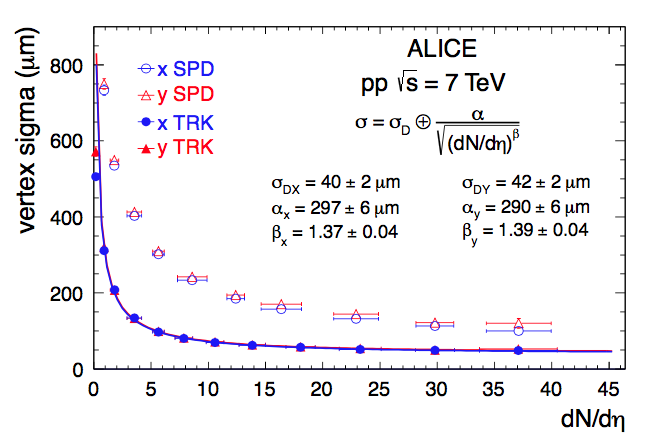
\includegraphics[width=.49\textwidth]{FigCap3/VtxReso.png}
\includegraphics[width=.49\textwidth]{FigCap3/DCAxyResol.png}
\caption{Left: resolution on the transverse coordinate of the vertex position from tracks (solid points) and SPD tracklets (open points) as a function of multiplicity~\cite{Abelev:2014ffa}. Right: resolution of the distance of closest approach to the primary vertex in the transverse plane for charged ITS-TPC tracks. The contribution from the vertex resolution is not subtracted~\cite{Abelev:2014ffa}. }
\label{fig:VtxResolDCAResol}
\end{figure}
\end{itemize}
\begin{figure}[!h]
\centering
\includegraphics[width=.49\textwidth]{FigCap3/ptResol.png}
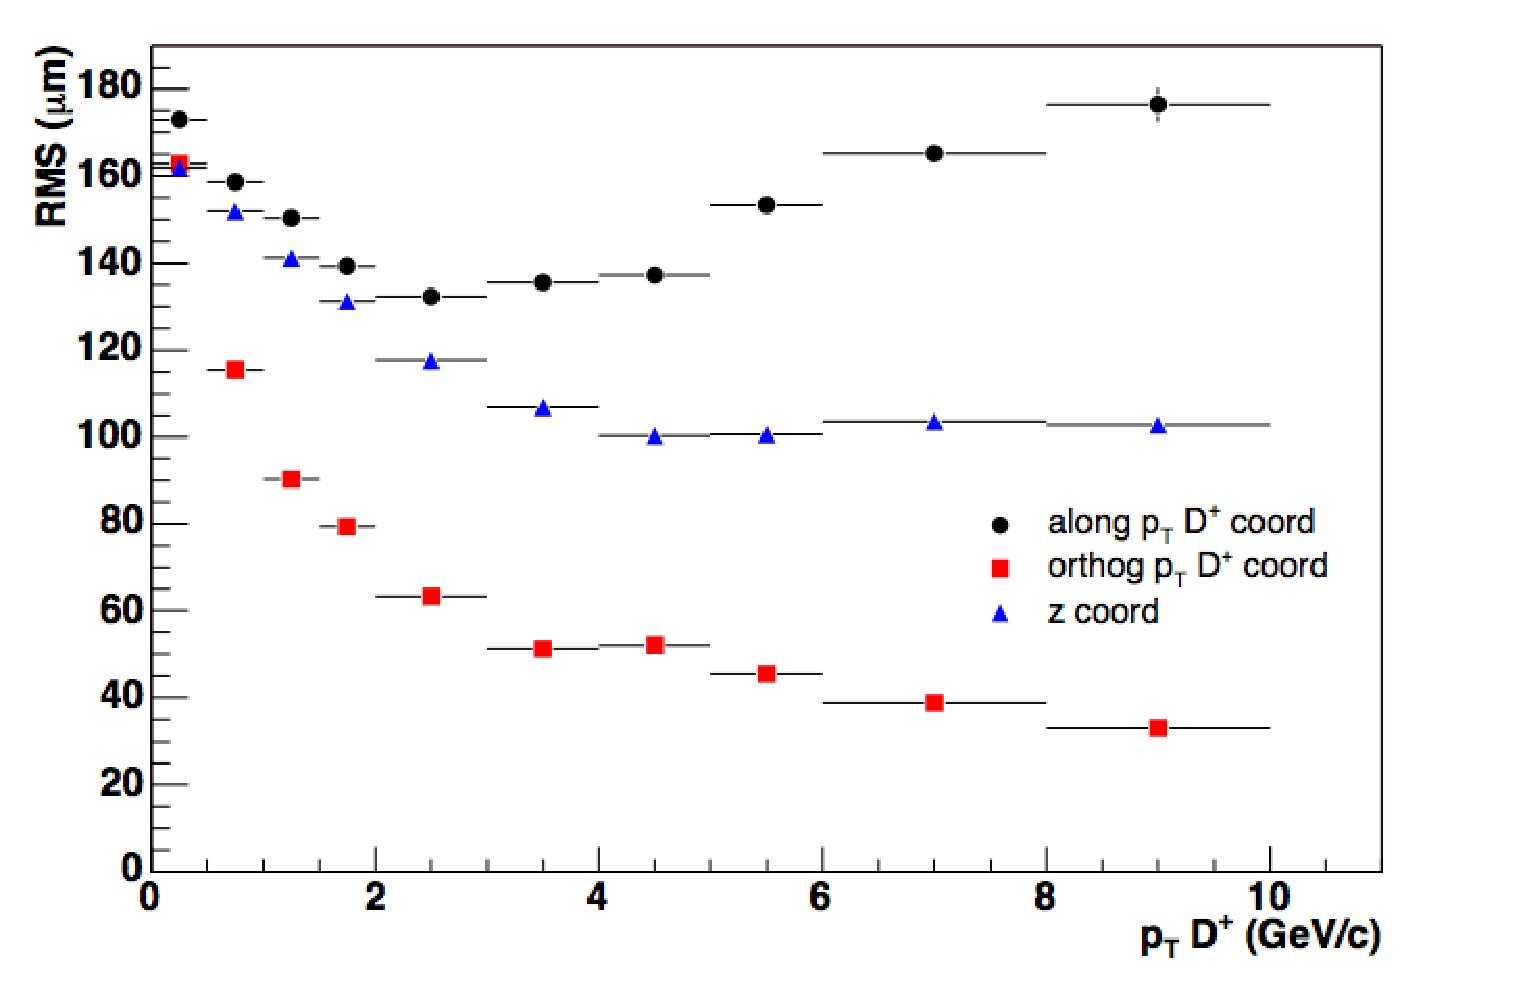
\includegraphics[width=.49\textwidth]{FigCap3/vertexSec.pdf}
\caption{Left: $\pt$ resolution for TPC standalone and ITS-TPC tracks with and without the constraint to the vertex~\cite{Abelev:2014ffa}. Right: resolution of the position of the reconstructed secondary vertex of $\DplustoKpipi$ decays along $\Dplus$ $\pt$ direction (black), 
orthogonal to $\Dplus$ $\pt$ direction (red), and along $z$-axis (blue).}
\label{fig:PtResolAndSecVtxResol}
\end{figure}

\section{Secondary vertex reconstruction}
\label{sec:secVertex}
For the reconstruction of heavy-flavour hadron decays, the reconstruction of decay vertices 
is done during the analysis phase. Tracks are grouped in pairs (e.g. for the $\DtoKpi$ decays) or in triplets (for the $\Dplus$ and $\Dsplus$ cases), 
defining objects called ``candidates''. 
The algorithm used for the secondary vertex reconstruction is based on a straight 
line approximation of the tracks (which are helices) in the vicinity of the primary vertex, by calculating the tangent line.
The algorithm finds the point of minimum distance between the two (or three) tracks by minimising the quantity:
\begin{equation}
D^2= \sum_{i=1}^N d_i^2,
\end{equation}
where N is the number of decay particles (3 in case of $\DstoKKpi$ decays) and $d_i$ is the distance between the track $i$ and the vertex 
($x_0$, $y_0$, $z_0$), weighted with the errors from the track covariance matrix:
\begin{equation}
d^2_i=\left(\frac{x_i-x_0}{\sigma_{x_i}}\right)^2+
\left(\frac{y_i-y_0}{\sigma_{y_i}}\right)^2+\left(\frac{z_i-z_0}{\sigma_{z_i}}\right)^2.
\end{equation}
The resolution of the reconstructed secondary vertex is shown in Fig.~\ref{fig:PtResolAndSecVtxResol} (right) 
(right) as example for the $\DplustoKpipi$ meson. The 
resolution improves with increasing $\Dplus$ meson $\pt$ and is better in the plane perpendicular to the $\Dplus$ $\pt$ direction.
The resolution of the secondary vertex for the $\DstoKKpi$ meson is similar to that of $\Dplus$.
Resolutions of about 100 $\mu$m allow to resolve the $\Ds$ decay vertices, which are
displaced from the interaction point by $\approx 150-300\,\mu$m.


\section{Simulations}
\label{sec:simu}
Simulations are used in the analysis to calculate the reconstructed efficiencies and to study the detector
performance.
Event generators are used to simulate pp, p-Pb and Pb-Pb collisions. In particular, PYTHIA 6 and
PYHTIA 8 were used for pp collisions, DPMJET, HIJING and EPOS-LHC for Pb-Pb and p-Pb collisions
for the studies presented in this thesis.
The physics processes at partonic level and informations such as type, momentum, 
charge, mother/daughter relationships... are stored in the kinematics tree. The GEANT package
is then used to simulate the transport of the particles through the
  detectors. During the transport, the energy deposition in the various detectors is stored 
  as ''hits''. The hits are subsequently converted into ''digits'', which represent 
  the real detector response and take into account instrumental effects, such as the presence of inactive channels, the noise 
  due to the front-end electronics ... The digits correspond to the raw data coming from the 
  Data Acquisition System in a real data taking. The same reconstruction procedure used for real data is applied to the simulated
  digits.

\section{Centrality determination}
\label{sec:centr}
The geometrical Glauber model~\cite{Miller:2007ri} introduced in Sec.~\ref{sec:glauber} describes
nuclear collisions as a superposition of binary nucleon-nucleon interactions. 
A participant nucleon of one nucleus is defined as a nucleon that undergoes one or more 
 collisions with nucleons of the other nucleus. The number of participants nucleons $N_{\rm part}$
 can be calculated as a function of the impact parameter $b$ of the collision using the Glauber
 model, the nucleon-nucleon inelastic cross section and the nucleon density profiles of the projectile and target
 nucleus. The number of spectator nucleons can be computed from the number of participant nucleons 
$N_{\rm part}$ as $N_{\rm spec}$ = $A_{\rm proj}$ + $A_{\rm target}$ - $N_{\rm part}$, where $A_{\rm proj}$ and $A_{\rm target}$
are the mass numbers of the colliding nuclei. The number of binary 
collisions $N_{\rm coll}$ can be calculated for a given value of the impact parameter. 
The impact parameter $b$ and other geometry-related quantities ($N_{\rm part}$, 
$N_{\rm spec}$, $N_{\rm coll}$) are not directly measurable. The determination of the collision centrality is based 
measurements of multiplicity (energy) produced in the collision, which can be described utilising
the Glauber model convoluted with a model for particle production based on a negative binomial distribution (NBD):
\begin{equation}
\label{eq:NBD}
P_{\mu, k} (n) = \frac{\Gamma(n+k)}{\Gamma(n+1)\Gamma(k)}\frac{(\mu/k)^n}{(\mu/k+1)^{n+k}},
\end{equation}
which gives the probability of measuring $n$ hits per independent emitting source of particles (called ancestor),
 where $\mu$ is the mean multiplicity per ancestor and $k$ controls the width of the distribution. 
The number of ancestors is parameterised as: $N_{\rm ancestors} = fN_{\rm part} + (1- f) N_{\rm coll}$.
This is inspired by two-component models~\cite{Deng:2010mv,Kharzeev:2004if}, which decompose particle production in nucleus-nucleus 
collisions into the contributions due to soft and hard interactions, where the soft interactions produce particles with 
an average multiplicity proportional to $N_{\rm part}$, and the probability for hard interactions to occur is proportional to $N_{\rm coll}$. 
\begin{figure}[!h]
\centering
\includegraphics[width=.52\textwidth]{FigCap3/v0glau_276.pdf}
\includegraphics[width=.46\textwidth]{FigCap3/zdczem.pdf}
\caption{Left: distribution of the sum of amplitudes in the V0 scintillators for events in Pb-Pb collisions at $\sNN=2.76$ TeV~\cite{Abelev:2013qoq}. The distribution is fitted with the NBD-Glauber fit, shown as a red line. The centrality classes used in the analysis are indicated in the figure. The inset shows a zoom of the most peripheral region. Right: spectator energy deposited in the ZDC calorimeters as a function of ZEM amplitude~\cite{Abelev:2013qoq}. The lines are a fit to the boundaries of the centrality classes with linear functions.}
\label{fig:centrality}
\end{figure}
%Two experimental observables related to the collision geometry are the average charged-particle 
%multiplicity $\Nch$ and the energy carried by particles close to the beam direction and 
%deposited in zero-degree calorimeters (ZDC). The average charged-particle multiplicity decreases
%monotonically with the impact parameter. 
With the Glauber Monte Carlo approach, the collision processes are simulated  
and the $N_{\rm part}$, $N_{\rm coll}$ and the number of ancestors are computed event by event. 
This allows to extract multiplicity distributions which can be compared to the measured ones and to extract the values of the parameters
$\mu, n $ and $k$.
The standard method typically used in ALICE is to define 
the centrality classes in Pb-Pb collisions based on the NBD-Glauber fit to the sum of V0A and V0C amplitudes. 
Other methods are used to asses the systematic uncertainty on the centrality determination~\cite{Abelev:2013qoq}.
In Fig.~\ref{fig:centrality} (left panel) the distribution of the V0 amplitudes for Pb-Pb collisions 
at $\sNN=2.76$ TeV~\cite{Abelev:2013qoq} is shown. The events were triggered with a signal in both V0A
and V0C and at least two hits in the outer SPD layer. The beam background was removed,
as well as part of the EM background with a ZDC cut and a $z$-vertex cut ($|\zVtx|<10$ cm).
The V0 amplitude obtained with the NBD-Glauber model fitted to the data is shown as a red curve
 in Fig.~\ref{fig:centrality} (left). The centrality is expressed as a percentage of the total nuclear interaction cross section
$\sigma$ obtained by integrating the V0
amplitude distribution. The normalisation is performed utilising the integral up to a threshold value V0$_{\rm THR}$ (anchor point), which corresponds
to the 90\% of the total hadronic cross section. For example, if we define V as the VZERO amplitude, 
the top 10\% central class is defined by the boundary V0$_{10}$ which satisfies:
\begin{equation}
\label{eq:percentileV0}
\frac{\int_{{\rm V0}_{\rm 10}}^\infty ({\rm d }N_{\rm ev} / {\rm d}V) {\rm d}V}{\int_{{\rm V0}_{\rm THR}}^\infty ({\rm d }N_{\rm ev} / {\rm d}V) {\rm d}V} = \frac{1}{9}.
\end{equation}
 Events with lower multiplicity than that of the anchor point
suffer from contamination of EM background and trigger inefficiencies, therefore are not used
in the determination of the centrality percentiles. The experimental distribution can be divided into classes by defining intervals on the measured distribution, 
which correspond to defined percentile intervals of the hadronic cross section. 
Another detector that can be used to determine the centrality of an event is the ZDC.
The energy deposited by the spectator nucleons in the ZDC has a monotonic dependence
on the multiplicity only for relatively small impact parameter values. For peripheral collisions, in particular,
it is possible that the nuclei fragments resulting from the collision have a magnetic rigidity (ratio
of their charge and mass) similar to that of beam particles, thus they are not bent away from the beam vacuum tube 
by the magnets and their energy is not
collected by the ZDCs. For this reason, the ZDC information needs to be correlated with the signals measured
by the two EM calorimeters (ZEM), as shown in the right panel of Fig.~\ref{fig:centrality}~\cite{Abelev:2013qoq}. 
The centrality classes previously determined 
by using the V0 are used to individuate the centrality classes in the ZDC-ZEM plane, since the ZEM
amplitude has unknown dependence on $N_{\rm part}$ and $N_{\rm coll}$. Then, the centrality classes 
are defined by cutting the plane into regions defined by straight lines from linear fits to the boundary regions
between two adjacent classes. This allows to define centrality intervals up to the 30\% of the hadronic cross section,
but not for more peripheral collisions.


\section{The ALICE Offline Software Framework}
\label{sec:offline}
In ALICE, pp and Pb-Pb events recorded with MB trigger have an average size of about 1.1MB and 13.75 MB respectively. 
For the Pb-Pb data sample at $\sNN=5.02$ TeV in 2015, a total raw data volume of 2.4 PB was collected; volumes of 500 TB and 2.7 PB
of raw data were collected for the p-Pb (2016, $\sNN=5.02$ TeV) and pp (2017, $\s=13$ TeV) data samples, respectively.
 The processing and analysis of these data necessitate 
unprecedented amount of computing and storage resources. Grid computing provides 
the answer to these needs. Grid computing consists of a coordinated use of large sets 
of different, geographically distributed resources in order to allow high-performance 
computation. It is organised in different levels or Tiers. Data coming from LHC experiments 
are stored in the CERN computing centre, the Tier-0. Copies of the collected data are then 
replicated in large regional computing centres (Tier-1), which also contribute in the event 
reconstruction and Monte Carlo simulation. Tier-2 centres are computing centres located
 in different institutions which do not have large storage capabilities but provide a large 
 fraction of the computing resources for Monte Carlo simulations and 
 data analysis. ALICE uses the ALICE Environment (AliEn) system~\cite{Saiz:2003wi} as a 
 user interface to connect to a Grid composed of ALICE specific services that are part 
 of the AliEn framework and basic services of the Grid middleware installed at the different sites.

\subsection{The AliRoot Framework}
\label{subsec:AliRoot}
The ALICE offline framework, AliRoot~\cite{Aamodt:2008zz} is based on Object-Oriented techniques
 for programming and, as a supporting framework, on the ROOT system~\cite{Brun:1997pa}, 
 complemented by the AliEn system which gives access to the computing Grid. The 
 AliRoot framework was developed as an extension of ROOT and is used for simulation, 
 alignment, calibration, reconstruction, visualisation and analysis of the experimental data.
\begin{figure}[h]
\centering
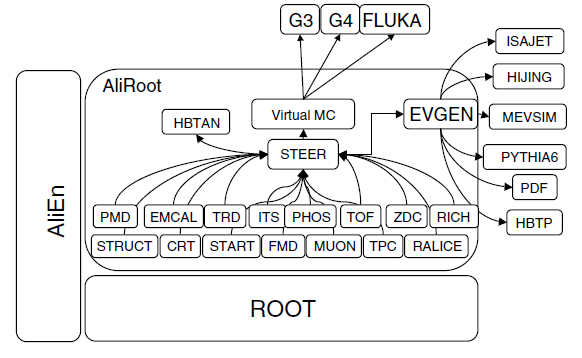
\includegraphics[width=10cm]{FigCap3/aliroot.png}
\caption{Schematic view of the AliRoot framework.}
\label{fig:aliroot}
\end{figure}
The AliRoot framework is schematically shown in Fig.~\ref{fig:aliroot}. The STEER module 
provides steering, run management, interface classes, and base classes. The detector related software is divided in 
independent modules that contain the code for simulation and reconstruction. Detector response simulation can be performed 
via different transport  packages like GEANT3~\cite{Brun:1082634} 
written in FORTRAN and GEANT4~\cite{Agostinelli:2002hh} written in C++. In these packages 
the detector material budget is simulated in detail, including support structures and 
the beam pipe. The transport code can hence simulate the decays of unstable 
particles and the trajectory of the daughter particles, the interactions of the 
particles with the detectors material and the production of secondary particles.
The reconstruction results are stored in ESDs (Event Summary Data), from which 
the AODs (Analysis Object Data) are extracted. The AODs contain the relevant information
for physics analyses. Additional information, used only for some specific analysis, is stored in additional
files, usually called delta-AODs. For example, specific AOD are produced for the 
reconstruction of open-charm meson with two or three body decays.
The analysis code, which contain the tasks utilised by the user to read the AOD files on the GRID and
to produce quantities, histograms and trees for final analysis, calculations of efficiencies and quality and
stability checks, is contained in the AliPhysics framework, which is built on the AliRoot and ROOT
frameworks and is progressively developed by the data analysis groups.
